% !TEX root = C:\Users\Jan\Documents\dev\Risk-Measurement-Framework\masterthesis_tex\masterthesis_main.tex
\section{Implementation}
\label{sec:implementation}

The technical RMF uses Python 3.7 as the programming language and ART as the basis. Beside the attacks given by the ART, there is a function from the technical RMF to execute individual attacks. This technical RMF should be used a step ahead of using the framework of Schwerdtner et al.

\subsection{Structure of the RMF}

\subsubsection*{Directory tree}

The RMF is structured as follows: \\

\dirtree{%
.1 rmf/.
.2 attacks/.
.3 art/.
.4 backdoors.py.
.2 backdoors/.
.3 png-Files.
.2 measurement/.
.3 monitoring.py.
.2 metrics/.
.3 log.py.
.2 visualizations/.
.3 plot.py.
.2 log\_file.log.
.2 case\_study.py.
}

\break \noindent The \textit{png-Files} are used by the \textit{backdoors.py} script to add patterns into the images that are the backdoor triggers. Both folders \textit{measurement} and \textit{metrics} contain implementations to monitor the collected data for the risk measurement and evaluate it. The \textit{visualizations} folder shows the measurement results and summarize them into one output file.

\subsection{Implement the risk indicatiors}

The risk indicators are the main part for the risk measurement. Therefore the risk indicators are used through the complete risk measurement. Every risk indicator is implemented as an own function in the RMF. This makes it possible to measure the risk indicator values at every step during the ML model training. The goal is to use measure the risk indicator values with the original training data and the manipulated training data. The $accuracy=\frac{n(correctly\_predicted)}{n(all)}$ is implemented as Nguyen and Zeigermann \cite{9783960101925} describe it. The next risk indicator is the attack time that checks when the attack execute. This can be during training or deployment time. Implementing this checks which attack is executed. Attack specificity is an risk indicator that measures if the attack is targeted or untargeted. This is a risk indicator that measures where the backdoor trigger is implemented. The ART attacks have a parameter that takes target. If the target is random, there is no specific label. If it is targeted, there is a specific label where a certain number of images in percentage are poisoned or specific images of a targeted label. Positive and negative label is a risk indicator that measures during training time the TP, TN, FP, FN. Keras show these values with a implemented function in this technical framework. The computational resources get the values from the operating system for the specific executed program. The attacker's knowledge is implemented based on the attack. For example, if the \textit{Pattern Backdoor Attack} is implemented in the ML model, then it returns the steps to implement this specific attack \cite{bsi_2013}. Attacker's goal \cite{DBLP:journals/corr/abs-2012-04884} can be an inference failure, obtain secret information, or executing a denial-of-service. The goal of this risk indicator is to evaluate it based on monitored data of the attack. So the attack must have characteristics that represent the goal an attacker has. An inference failure happens during the testing phase. So when an attacker try to execute an inference failure he could use exploratory attacks \cite{tabassi2019taxonomy}. Obtain secret information can be for example stealing model attacks \cite{DBLP:journals/corr/abs-2105-00623}, \cite{DBLP:journals/wicomm/ZhangLGQTZ20}. Denial-of-service attacks have the goal to slow down the ML model or crash the ML model completly \cite{DBLP:journals/sensors/VaccariAC20}.

\subsection{Implementing backdoor attacks from the ART}

The following three attacks are all based on the ART \cite{art2018} and represent white-box and black-box attacks and both targeted and untargeted attacks. These attacks are the main factor to assign the values to the base measures. The attacks already differentiate between the original and poisoned dataset for evaluation.

\subsubsection*{Backdoor attacks from the ART}
\label{sec:backdoors_art}

All backdoor attacks use the \textit{Pattern Backdoor Attack} \cite{DBLP:journals/corr/abs-1708-06733} class which expects a pattern argument. The pattern is a picture which is for the poisoned images in the training data. The pattern must be implemented before training and choose a random selection of images. This is implemented in the RMF as follows:

\begin{lstlisting}
  n_train = np.shape(x)[0]
  num_selection = num_of_rand_images
  random_selection = np.random.choice(n_train, num_selection)
  x = x[random_selection]
  y = y[random_selection]
\end{lstlisting}

Then the arguments $x$ and $y$ are passed to the poisoning function from the ART. $x$ and $y$ are parameters which the function expects when calling it. Appendix \ref{sec:frame_func} describe the functions and parameters. Further it is important that the shape of the images from the training data are \textit{N, H, W, C} or \textit{N, C, H, W}. $N$ is the number of images in the batch, $H$ is the image height, $W$ is the image width, and $C$ is the channel number of an image such as grayscale or RGB. After adding a backdoor as a pattern to the random images, the poisoned images are replaced back to the training data. These poisoned images are saved in a different folder to check if the images are missclassified after or while testing the ML model.\\

The first attack uses the \textit{Pattern Backdoor Attack} class without any other backdoor classes from the ART. This attack which bases on Gu et al. \cite{DBLP:journals/corr/abs-1708-06733} is a black-box attack which is untargeted. In the RMF it uses a pattern backdoor which Figure \ref{fig:original_example} and Figure \ref{fig:poisoned_example} show as the difference between the original and the poisoned image. The goal of this attack is to change the original label to a random other label. This attack can be executed without any information because it is not important which training data the ML model use and what ML model is used for the training itself.

\begin{figure}[!tbp]
  \centering
  \begin{minipage}[b]{0.4\textwidth}
    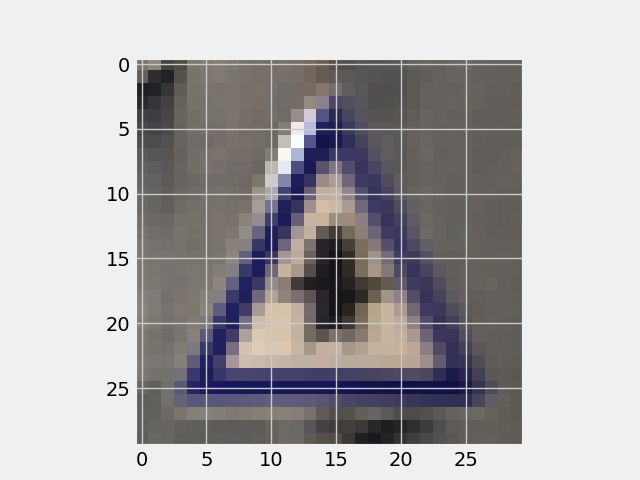
\includegraphics[width=8cm]{pictures/original_example.png}
    \caption{Street sign without a backdoor pattern with the label \textit{Right-of-way at intersection}}
    \label{fig:original_example}
  \end{minipage}
  \hfill
  \begin{minipage}[b]{0.4\textwidth}
    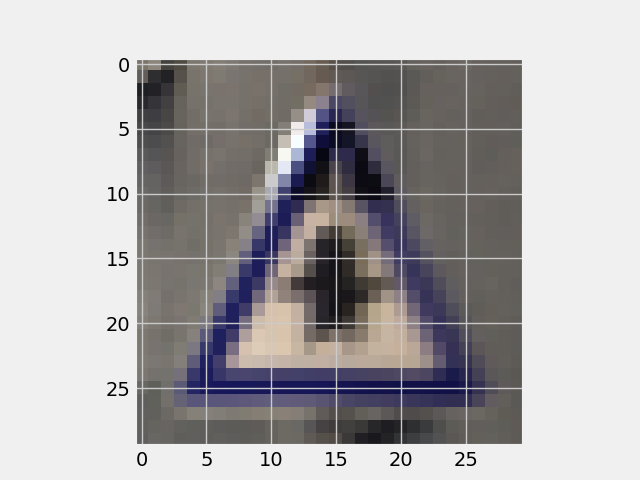
\includegraphics[width=8cm]{pictures/poisoned_example.png}
    \caption{Street sign with a backdoor pattern but still with the original label \textit{Right-of-way at intersection}}
    \label{fig:poisoned_example}
  \end{minipage}
\end{figure}

After poisoning the images these image need be copied back into the original training data. Before this can be done the poisoned data must replace the original training data which contain no backdoor. When the RMF take the random original images, it save them into a temporary variable and then delete the images from the original training data. The next step is the poisoning while the poisoned data and the original training data need the same shape and dimension which make it possible to copy the poisoned images. As mentioned before the poisoning function takes only two specific shapes which make it easy to have the same shape in the original training data and poisoned data. The implementation of the attack additionally shows the effort an attacker have to implement this attack. Thus the steps can be used for the attacker's knowledge risk indicator.

The \textit{Clean Label Backdoor Attack} \cite{turner2018clean} poison images and misclassify during the training time. To use this attack the \textit{Pattern Backdoor Attack} must be used before and then the clean label attack can be executed after training. After adding the backdoor trigger with \textit{Pattern Backdoor Attack} the original training data are trained with a proxy classifier which should do the same classification tasks as the original classifier. The first poison step is selecting target images. As next the PGD (which is untargeted) must be implemented to make it harder classify correctly. The last step is adding the backdoor trigger and add the target label.

The \textit{Hidden Trigger Backdoor Attack} \cite{DBLP:journals/corr/abs-1910-00033} need to be executed after training. To add the backdoor, the \textit{Pattern Backdoor Attack} must be used before. After training the poisoned data and a smaller number of clean training inputs are used to finetune the model. Finetuning means, taking a equal number of training inputs from each label. The following Python code shows the finetuning of a ML model where the attack is implemented.

\begin{lstlisting}
  dataset_size = size
  num_labels = label_size
  num_per_label = dataset_size/num_labels

  poison_dataset_inds = []

  for i in range(num_labels):
      label_inds = np.where(np.argmax(y_train, axis=1) == i)[0]
      num_select = int(num_per_label)
      if np.argmax(target) == i:
          num_select = int(num_select - min(num_per_label, len(poison_data)))
          poison_dataset_inds.append(poison_indices)

      if num_select != 0:
          poison_dataset_inds.append(np.random.choice(label_inds, num_select, replace=False))

  poison_dataset_inds = np.concatenate(poison_dataset_inds)

  poison_x = np.copy(x_train)
  poison_x[poison_indices] = poison_data
  poison_x = poison_x[poison_dataset_inds]

  poison_y = np.copy(y_train)[poison_dataset_inds]
\end{lstlisting}

The implementation of the \textit{Hidden Trigger Backdoor Attack} is analogous to the \textit{Clean Label Backdoor Attack} but it takes a different pattern as the backdoor trigger which Figure \ref{fig:poisoned_hidden_trigger} shows.

\begin{figure}[ht!]
  \centering
  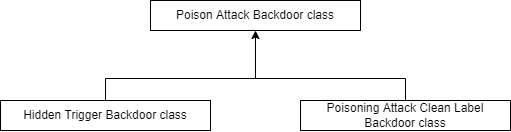
\includegraphics[width=9cm]{pictures/attack_relationship.png}
  \caption{Both attack classes (\textit{Clean Label Backdoor Attack} and \textit{Hidden Trigger Backdoor Attack}) get the backdoor from the \textit{Pattern Backdoor Attack}}
  \label{fig:relation_risk_ind}
\end{figure}

\subsection{The logging function}

Assigned values of the risk indicators are represented with an optimized logging function, based on the Python logging module. The function waits for two parameters. A message string and the wanted logging level (i.e. INFO or DEBUG). The called log function in the RMF could look like this:
\begin{lstlisting}
  log(f"{variable_name}", 'INFO')
\end{lstlisting}

In order not to depend on the different ML libraries the rmf gets its own functions of the different metrics. That increases the support of different Python libraries for ML risk
measurement.

\subsection{Using the threat model}
The measurement methods are implemented based on the threat model of Doynikova et al. \cite{DBLP:conf/crisis/DoynikovaNGK20}.
\subsection{Evaluation with the measurement construct of ISO 27004}

After assigning the risk indicators based on the threat model of Doynikova et al. \cite{DBLP:conf/crisis/DoynikovaNGK20}, this subsection explains the implemented measurement construct starting from the base measures up to the decision criteria. \\

\subsection{Show the measurement results}

The measurement results show the monitored data based on ISO 27004 \cite{ISO_27004_2009}. The second part shows the risk for the ML model with an attack. A risk matrix divides the risk in a specific part of the matrix. The risk matrix is based on the concept of risk. The risk is calculated by multiply the extent of damage with the probability of occurrence. The result of this is classified in the risk matrix.
